\documentclass{beamer}

\usepackage{graphicx}
%\usepackage{minted}

\title{The Measurement of Anisotropic Thermal Conductivity in Snow With Needle Probes}
\subtitle{A Thesis Defense}
\author{Joshua Holbrook}
\date{April 4th, 2011}

\begin{document}
\frame{\titlepage}


\begin{frame}
\frametitle{Why Do We Study Snow's Thermal Conductivity?}
\begin{columns}[c]
\column{0.5\textwidth}
     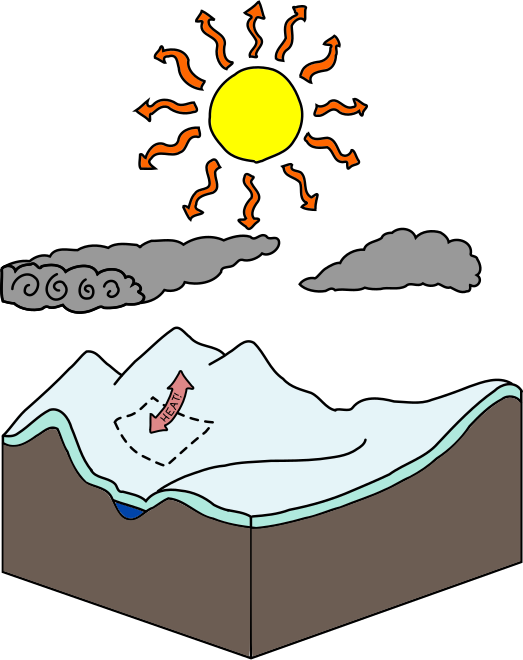
\includegraphics[width=\textwidth]{fig/climate.png}
\column{0.5\textwidth}
    \begin{itemize}
    \item Climatologists want to model Arctic climates.
    \item Heat transfer occurs between the earth and the atmosphere.
    \item Snow gets in the way.
    \end{itemize}
\end{columns}
\end{frame}


\begin{frame}
\frametitle{How Do We Measure Thermal Conductivity?}
    \begin{itemize}
    \item One way is a guarded hot plate.
    \item Steady state 1-D conduction: \(k = \frac{\dot{q}l}{A\Delta T}\)
    \item Guarded hot plates are good for measuring foam boards.
    \item Guarded hot plates aren't exactly ideal for snow.
    \end{itemize}
\end{frame}


\begin{frame}
\frametitle{There HAS to be a better way.}
\begin{columns}[c]
\column{0.5\textwidth}
     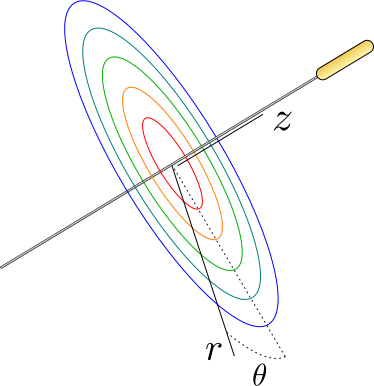
\includegraphics[width=\textwidth]{fig/basic_geometry.png}
\column{0.5\textwidth}
    \begin{itemize}
    \item It's called a needle probe.
    \item It looks something like this.
    \item It does \emph{not} use steady-state conduction.
    \item It depends on a \emph{radial} geometry.
    \end{itemize}
\end{columns}
\end{frame}

\end{document}


